

\preClass{Linear Theory}

\begin{problem}
\item Find the solution to the following differential equation
  \begin{eqnarray}
    \label{eqn:nonhomogeneousPreClass}
    y' + ty & = & e^{-t}.
  \end{eqnarray}

  \begin{subproblem}
  \item First find a solution to the homogeneous equation
  \begin{eqnarray*}
    y_h' + ty_h & = & 0.
  \end{eqnarray*}

      \iftoggle{solutions}{%

        \begin{eqnarray*}
          y'_h & = & -t y_h, \\
          \frac{y'_h}{y_h} & = & -t, \\
          \ln\lp y_h \rp & = & -\half t^2 + C, \\
          y_h & = & k e^{-t^2/2}.
        \end{eqnarray*}
        
      }

    \vfill

  \item Assume that the solution to equation
    \ref{eqn:nonhomogeneousPreClass} is in the form $y(t) = u(t)
    y_h(t)$ where $y_h(t)$ is your solution to the homogenous
    equation. Take the derivative of $y(t)$. (Use the product rule!)

      \iftoggle{solutions}{%

        \begin{eqnarray*}
          y & = & u \cdot y_h, \\
          y' & = & u' y_h + u y_h'.
        \end{eqnarray*}
        
      }{%

        \vspace*{6em}

      }


    (See the next page.)
    \clearpage

  \item Substitute the function $y(t)$ into the original differential
    equation and solve for $u(t)$. (Do not forget the ``+C'' after
    integrating.)

      \iftoggle{solutions}{%

        \begin{eqnarray*}
          u' y_h + u y_h' + t u y_h & = & t, \\
          u' k e^{-t^2/2} + u (-t) k e^{-t^2/2} + t u k e^{-t^2/2} & = & t, \\
          u' k e^{-t^2/2} & = & t, \\
          u' & = & \frac{1}{k} e^{t^2/2} + C.
        \end{eqnarray*}
        
      }

      \vfill

  \item Substitute the solution, $u(t)$, into your definition,
    $y=u\cdot y_h$, to get the solution to the differential equation.

      \iftoggle{solutions}{%

        \begin{eqnarray*}
          u y_h & = & k e^{-t^2/2} \lp \frac{1}{k} e^{t^2/2} + C \rp, \\
          & = & 1 + \bar{C} e^{-t^2/2}
        \end{eqnarray*}
        
      }{%

        \vspace*{6em}

      }


  \end{subproblem}
\end{problem}


  \actTitle{Growth and Decay}
  \begin{problem}
  \item Find the solution to the following differential equation:
    \begin{eqnarray*}
      A' & = & -0.1 A, \\
      A(0) & = & 1000.
    \end{eqnarray*}
    What is the long term solution?

      \iftoggle{solutions}{%

        \begin{eqnarray*}
          \frac{A'}{A} & = & -0.1, \\
          \ln(A) & = & -.1 t + C, \\
          A & = & k e^{-.1 t}, \\
          A(0) & = & 1000, \\
          1000 & = & k e^0, \\
          A(t) & = & 1000 e^{-.1t}.
        \end{eqnarray*}

        In the long term
        \begin{eqnarray*}
          \lim_{t \rightarrow \infty} A(t) & = & 0.
        \end{eqnarray*}

      }

    \vfill
    \clearpage
  \item The number of bacteria in a colony at 10:00am is approximately
    five million. At noon the number is approximately seven
    million. How many bacteria were in the colony at 9:00am?

      \iftoggle{solutions}{%

        We denote the number of bacteria in the dish at time to be
        $B(t)$. We assume that 10:00am is time zero. The governing
        equation and the solution follow:

        \begin{eqnarray*}
          B' & = & r B, \\
          \Rightarrow B & = & ke^{rt}, \\
          B(0) & = & 5,000,000, \\
          & = & k e^0, \\
          B(t) & = & 5,000,000 e^{rt}, \\
          B(2) & = & 7,000,000, \\
          & = & 5,000,000 e^{2r}, \\
          \frac{7}{5} & = & e^{2r}, \\
          2r & = & \ln(7/5), \\
          r & = & \half \ln(7/5), \\
          B(-1) & = & 5,000,000 e^{-1 \cdot \half \ln(7/5)}, \\
          & \approx & 4,225,771.
        \end{eqnarray*}

      }

    \vfill
  \end{problem}


  \actTitle{Mixing}
  \begin{problem}

  \item A tank initially contains 2,000 litres of water with a
    concentration of mercury of $6.0\times 10^{-5}$ grams per
    litre. Water that contains $3.0\times 10^{-5}$ grams per litre is
    pumped into the tank at 100 litres per hour. The well mixed
    solution is pumped out of the tank at 100 litres per hour.  How
    long will it take for the concentration in the tank to reach
    $4.5\times 10^{-5}$ grams per litre?

    \begin{subproblem}
      \item Draw a picture. Label and define the important quantities.

        \iftoggle{solutions}{%

          \includegraphics[width=20em]{img/tankProblem}

        }{%

          \vfill

        }

      \item Define the quantity to use. Determine the rate that
        mercury moves into the tank, and determine the rate that
        mercury moves out of the tank. Define the initial condition.

        \iftoggle{solutions}{%

          The amount of mercury in the tank at time $t$ is denoted by $A(t)$.

          \begin{eqnarray*}
            \mathrm{rate~in} & = & 3\times10^{-5} \frac{g}{l} \cdot 100 \frac{l}{hr}, \\
            & = & 3\times10^{-3} \frac{g}{hr}.
          \end{eqnarray*}

          \begin{eqnarray*}
            \mathrm{rate~out} & = & A(t) g \cdot \frac{1}{2000~l} \cdot 100 \frac{l}{hr}, \\
            & = & A \cdot \frac{1}{20} \frac{g}{hr}.
          \end{eqnarray*}

          \begin{eqnarray*}
            A(0) & = & 2000~l \cdot 6\times 10^{-5} \frac{g}{l}, \\
            & = & 12\times10^{-2} ~g.
          \end{eqnarray*}

        }

        \vfill

        \clearpage

      \item Write out the differential equation and solve it to find
        the amount of mercury in the tank at any time. Once you find a
        formula for the amount of mercury determine the formula for
        the concentration at any time.

        \iftoggle{solutions}{%

          \begin{eqnarray*}
            A' & = & 3\times10^{-3} - \frac{1}{20} A, \\
            A' + \frac{1}{20} A & = & 3\times10^{-3}, \\
            A' e^{t/20} + \frac{1}{20} e^{t/20} A & = & 3\times10^{-3} e^{t/20}, \\
            \frac{d}{dt} \lp A e^{t/20} \rp & = & 3\times10^{-3} e^{t/20}, \\
            A e^{t/20} & = & 6\times10^{-2 } e^{t/20} + C, \\
            A & = & 6\times10^{-2} + C e^{-t/20}, \\
            A(0) & = & 12\times10^{-2}, \\
            12\times10^{-2} & = & 6\times10^{-2} + C, \\
            C & = & 6\times10^{-2}, \\
            A & = & 6\times10^{-2} + 6\times10^{-2} e^{-t/20}. \\
          \end{eqnarray*}

          The concentration is found by dividing by the volume,
          \begin{eqnarray*}
            \mathrm{Concentration} & = & \frac{6\times10^{-2} + 6\times10^{-2} e^{-t/20}}{2000}.
          \end{eqnarray*}

        }

        \vfill
        

    \end{subproblem}



\end{problem}
